\section{Conventions}
\label{sec:conventions}

Italic is used for scalars and vectors: {\em{$p$}}, $q$.
It is easy to distinguish which are which by context.
Bold maths is used for rank 2 tensors:
$\tenrtwo{I}$,
$\tenrtwo{R}$,
$\tenrtwo{\sigma}$.
Script is used for rank 4 tensors:
$\tenrfour{C}$.

`$\cdot$' denotes dot product, single contraction:
$x^s=\mathbold{R}^c \cdot x^c$.

`:' denotes double product, double contraction:
$\tenrtwo{\sigma} = \tenrfour{C} : \tenrtwo{\epsilon}$.

`$\otimes$' denotes tensor product:
$\mathbold{I}\otimes\mathbold{I}=
\delta_{ij}\delta_{kl}$.

\subsection{Space coarray}
\label{sec:space:coarray}

The space coarray is the centre part of the whole
library.
The idea is that 3D space is partitioned into identical
cells of some sort.
The cells are used to store and update some physically
relevant properties.
An important consideration is how many properties can
a cell store.
At present the coarray is defined as shown in
Eqn. \eqref{eq:coarray}:

\begin{equation}
\texttt{
coarray(l1:u1,l2:u2,l3:u3,props)[col1:cou1,col2:cou2,col3:*]
}
\label{eq:coarray}
\end{equation}
%
where \texttt{l1}\ldots\texttt{u3}
are the lower and the upper
spatial bounds of the array, counted in cells;
\texttt{props} is the number of properties a cell should
hold; \texttt{col1}\ldots\texttt{col3} are the lower
and the upper cobounds of the coarray.
Note that the last codimension is never specified,
i.e. it is always left as an asterix, \texttt{*}, to
allow for different number of images at runtime.

A typical definition of the coarray might look like

\begin{equation}
\texttt{
coarray(1:10,1:10,1:10,2)[1:8,1:8,1:*]
}
\nonumber
\end{equation}
%
which, when run on 512 images, will have the final
codimension of 8.
This array has 2 cell state types, which can be e.g.
the (unique) grain number, and a possible fracture state.

The library has two state types defined:
\texttt{cgca\_state\_type\_grain} for grain states,
i.e. grain numbers, and
\texttt{cgca\_state\_type\_frac} for fracture states.
So \texttt{coarray(:,:,:,cgca\_state\_type\_grain)} is
the local grain array, and
\texttt{coarray(:,:,:,cgca\_state\_type\_frac)} is
the local fracture array.

\subsection{Cellular neighbourhood}

We use a square 3D cellular array.
This means that a cell has a
$3 \times 3 \times 3 - 1 = 26$
cell nearest neighbourhood.
There are a number of problems with such
neighbourhood.
Not all neighbouring cells are `equal'.
If one imagines a $3\times 3 \times 3$ cube
of cubic cells, then the central cell will
have 6 neighbours sharing a face with it,
12 neighbours sharing an edge and 8 neighbours
sharing an edge.
More importantly, there are
three distinct angles between the pairs of the
nearest neighbourhood vectors, i.e. vectors
connecting the centres of the central cell,
and of each neighbouring cell \cite{shterenlikht2013c}.

Perhaps a better idea of a neighbourhood can
be constructed by imagining the central cell
as a 26-faced polyhedra.
Examples are rhombicuboctahedron or
pseudo-rhombicuboctahedron, also called
elongated square gyrobicupola, Johnson solid
J37, see Fig. \ref{fig:j37}.

\begin{figure}
\begin{tabular}{cc}
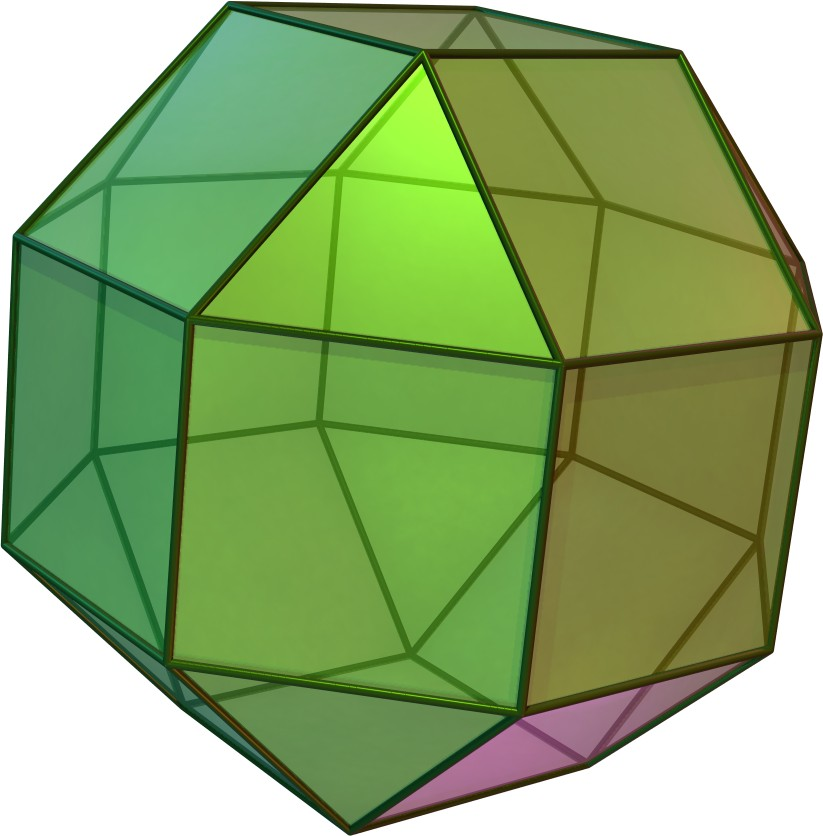
\includegraphics[width=0.4\textwidth]{octa.jpg}
&
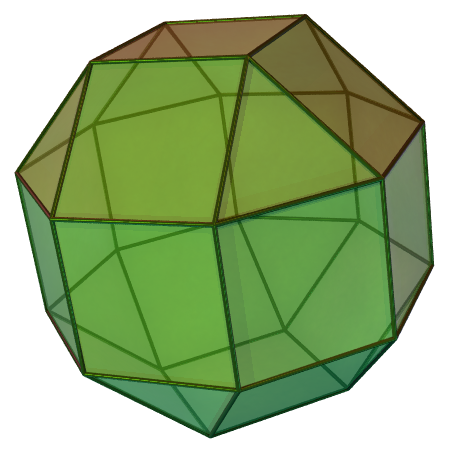
\includegraphics[width=0.4\textwidth]{gyro.png}
\\
(a) & (b)
\end{tabular}
\caption{
26-face polyhedra: (a) Rhombicuboctahedron, an Archimedian
solid, (b) Elongated square gyrobicupola, or
pseudo-rhombicuboctahedron, Johnson solid, J37.
From: http://en.wikipedia.org/wiki/Rhombicuboctahedron and
http://en.wikipedia.org/wiki/Elongated\_square\_gyrobicupola.
}
\label{fig:j37}
\end{figure}

Importantly, the cell state is determined
by the states of its neighbours, not the
other way round.
This helps develop a parallel model using
halo arrays.

